\documentclass[article]{jss}
\usepackage[utf8]{inputenc}
\usepackage[nogin]{Sweave}
\usepackage{pdfpages}
\usepackage{xspace}
\usepackage{tikz}
\usetikzlibrary{shapes.geometric, arrows}

\tikzstyle{io} = [trapezium, trapezium left angle=70, trapezium right angle=110, minimum width=3cm, minimum height=1cm, text centered, draw=black, fill=blue!30]
\tikzstyle{process} = [rectangle, minimum width=3cm, minimum height=1cm, text centered, draw=black, fill=orange!30]
\tikzstyle{decision} = [diamond, minimum width=3cm, minimum height=1cm, text centered, draw=black, fill=green!30]
\tikzstyle{arrow} = [thick,->,>=stealth]


\newcommand{\hl}[1]{\textcolor{magenta}{#1}}
\newcommand{\R}{\proglang{R}\xspace}

%%%%%%%%%%%%%%%%%%%%%%%%%%%%%%
%% declarations for jss.cls %%%%%%%%%%%%%%%%%%%%%%%%%%%%%%%%%%%%%%%%%%
%%%%%%%%%%%%%%%%%%%%%%%%%%%%%%

%% almost as usual
\author{Anne Helby Petersen\\Biostatistics\\Department of Public
  Health\\University of Copenhagen \And Claus Thorn Ekstr\o m\\Biostatistics\\Department of Public
  Health\\University of Copenhagen}
\title{\pkg{cleanR}: Maid for Cleaning Datasets in \proglang{R}}

%% for pretty printing and a nice hypersummary also set:
\Plainauthor{Anne Helby Petersen, Claus Thorn Ekstr\o m} %% comma-separated
\Plaintitle{{cleanR}: maid for cleaning datasets in R} %% without formatting
\Shorttitle{\pkg{cleanR}: maid for cleaning datasets in R} %% a short title (if necessary)

%% an abstract and keywords
\Abstract{Data cleaning and validation is the first step in any data
  analysis since the validity of the conclusions from the analysis
  hinged on the quality of the input data. Ideally, a human investigator
  should go through each variable in the dataset and look for
  potential errors --- both in input values and coding.

  We describe an \proglang{R} package which implements an extensive
  and customizeable suite of checks to be applied to the variables in
  a dataset in order to identify potential problems in the
  corresponding variables. The typical output is a stand-alone
  document that summarizes the variables and lists potential
  errors. The results are typically presented in a stand-alone
  document that could be perused by an investigator with an
  understanding of the variables in the data and the experimental design.

  The \pkg{cleanR} package is designed to be easily extended with custom
  user-created checks that are relevant in particular situations.
}
\Keywords{data cleaning, quality control, \proglang{R}}
\Plainkeywords{data cleaning, quality control, R} %% without formatting
%% at least one keyword must be supplied

%% publication information
%% NOTE: Typically, this can be left commented and will be filled out by the technical editor
%% \Volume{50}
%% \Issue{9}
%% \Month{June}
%% \Year{2012}
%% \Submitdate{2012-06-04}
%% \Acceptdate{2012-06-04}

%% The address of (at least) one author should be given
%% in the following format:
\Address{
  Claus Thorn Ekstr\o m\\
  Biostatistics, Department of Public Health\\
  University of Copenhagen\\
  Denmark\\
  E-mail: \email{ekstrom@sund.ku.dk}\\
  URL: \url{http://staff.pubhealth.ku.dk/~ekstrom/}
}
%% It is also possible to add a telephone and fax number
%% before the e-mail in the following format:
%% Telephone: +43/512/507-7103
%% Fax: +43/512/507-2851

%% for those who use Sweave please include the following line (with % symbols):
%% need no \usepackage{Sweave.sty}

%% end of declarations %%%%%%%%%%%%%%%%%%%%%%%%%%%%%%%%%%%%%%%%%%%%%%%


\begin{document}

\section{Introduction}
Statisticians and data analysts spend a large portion of their time on
data cleaning and on data wrangling. Packages such as
\pkg{data.table}, and \pkg{plyr} have made data wrangling a lot easier in
\proglang{R}, but there are only a few options available for automated data
cleaning.

Data cleaning is a time consuming endeavour and it inherently requires
human interaction since every dataset is different and the variables
in the dataset can only be understood in the proper context of the
experiment. While each dataset is different and requires unique
attention there are often a number of similar tasks that are
undertaken as part of the data cleaning and quality control
process. This is especially true when data are received repeatedly
from the same source as data providers tend to use a stable setup (and
hence introduce the same set of potential mistakes that need to be
identified and corrected).

In many situations these errors are discovered in the process of the
data analysis (e.g., a categorical variable with numeric labels is
wrongly classified as a numeric variable), but in other cases a human
with knowledge about the data context area is needed to identify
possible mistakes in the data (e.g., if there are 4 categories for a
variable that should only have 3).  It is necessary to summarize
information --- both numerically and graphically --- about each
variable in order for an investigator to detect possible errors, and
help raise flags of warning to draw the attention of investigator for
the situations where there \emph{might} be a error.

The \pkg{cleanR} package supports the automated checking of errors in
a dataset and produces an output document with detailed information
about each variable that can be
The process is illustrated in Figure~\ref{fig:flowchart1}. A dataset
is cleaned and an \proglang{R} markdown file is produced and possibly
rendered into html or pdf.

\begin{figure}
\begin{center}
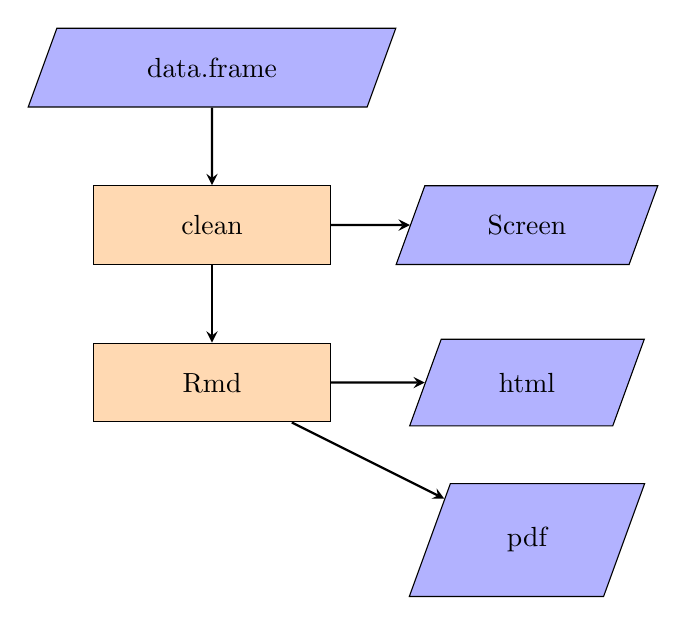
\begin{tikzpicture}[node distance=2cm]
\node (start) [io] {data.frame};
\node (pro1) [process, below of=start] {clean};
\node (screen) [io, right of=pro1, xshift=2cm] {Screen};
\node (pro2) [process, below of=pro1] {Rmd};
\node (html) [io, right of=pro2, xshift=2cm] {html};
\node (pdf) [io, below of=html] {pdf};
\draw [arrow] (start) -- (pro1);
\draw [arrow] (pro1) -- (screen);
\draw [arrow] (pro1) -- (pro2);
\draw [arrow] (pro2) -- (html);
\draw [arrow] (pro2) -- (pdf);
\end{tikzpicture}
\end{center}
\label{fig:flowchart1}
\caption{The process of cleaning data frames using the \pkg{cleanR}
  package. A series of check is applied to each variable in a
  \texttt{data.frame} and a summary of the result is either printed to
  the screen, or an \proglang{R} markdown file is produced which is
  subsequently rendered.}
\end{figure}


The manusccript is organized as follows. Section \ref{sec:example1}
presents a worked example and tutorial on how to use the \pkg{cleanR}
package to create a summary of potential errors. Section
\ref{sec:internals} presents the steps that comprise the creation of
the automated data cleaning that is part of the \code{clean} function,
while the \ref{sec:extending} Section explains how the set of checks
and graphical visualisations that are part of the cleaning suite are
extended by custom, used-written additions. Finally, plans for
extending the package are described in Section \ref{sec:conclusion}.


%% include your article here, just as usual
%% Note that you should use the \pkg{}, \proglang{} and \code{}
%% commands.


\section{Checking a dataset for errors} \label{sec:example1}

In \pkg{cleanR} the \code{clean} function is the primary workhorse and it
should be the primary entry point for data cleaning.

First we
\begin{Schunk}
\begin{Sinput}
> library(cleanR)
> data(diamonds)
> head(diamonds)
\end{Sinput}
\begin{Soutput}
  carat       cut color clarity depth table price    x    y    z
1  0.23     Ideal     E     SI2  61.5    55   326 3.95 3.98 2.43
2  0.21   Premium     E     SI1  59.8    61   326 3.89 3.84 2.31
3  0.23      Good     E     VS1  56.9    65   327 4.05 4.07 2.31
4  0.29   Premium     I     VS2  62.4    58   334 4.20 4.23 2.63
5  0.31      Good     J     SI2  63.3    58   335 4.34 4.35 2.75
6  0.24 Very Good     J    VVS2  62.8    57   336 3.94 3.96 2.48
\end{Soutput}
\begin{Sinput}
> data(testData)
> #head(testData)
\end{Sinput}
\end{Schunk}

To produce summary data-cleaning document

\begin{Schunk}
\begin{Sinput}
> clean(testData, replace=TRUE, openResult=FALSE)
\end{Sinput}
\end{Schunk}

By default, a ... is produced and the result is shown in
Figure~\ref{fig:example1}.

\begin{figure}[!htp]
\begin{center}
\includegraphics[page=2]{cleanR_testData.pdf}
%\includepdf[pages={2}, pagecommand={}]{cleanR_testData.pdf}
\end{center}
\label{fig:example1}
\caption{Example output from running XXXX on the testData
  dataset. First a summary of the full dataset, }
\end{figure}

Arguments


\section{The structure of cleanR} \label{sec:internals}


\begin{figure}
\begin{center}
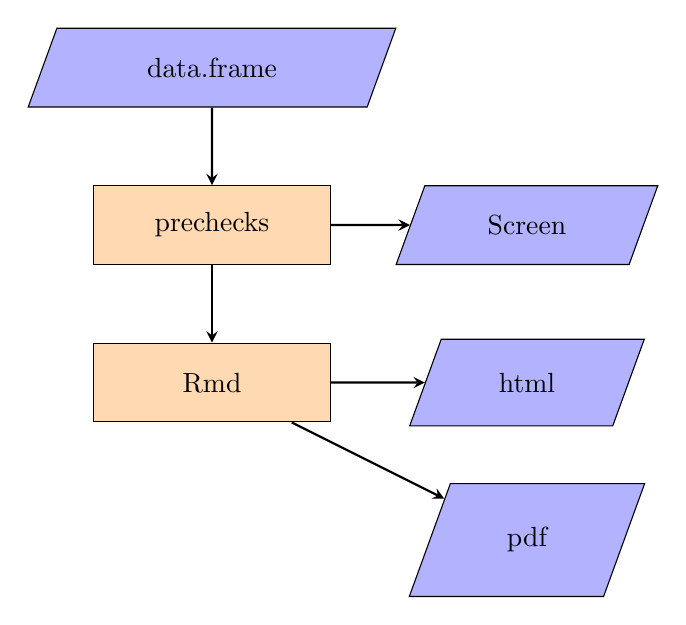
\begin{tikzpicture}[node distance=2cm]
\node (start) [io] {data.frame};
\node (pro1) [process, below of=start] {prechecks};
\node (screen) [io, right of=pro1, xshift=2cm] {Screen};
\node (pro2) [process, below of=pro1] {Rmd};
\node (html) [io, right of=pro2, xshift=2cm] {html};
\node (pdf) [io, below of=html] {pdf};
\draw [arrow] (start) -- (pro1);
\draw [arrow] (pro1) -- (screen);
\draw [arrow] (pro1) -- (pro2);
\draw [arrow] (pro2) -- (html);
\draw [arrow] (pro2) -- (pdf);
\end{tikzpicture}
\end{center}
\label{fig:flowchart1}
\caption{The process of cleaning data frames using the \pkg{cleanR}
  package. A series of check is applied to each variable in a
  \texttt{data.frame} and a summary of the result is either printed to
  the screen, or an \proglang{R} markdown file is produced which is
  subsequently rendered.}
\end{figure}

Bør vise DF -> prechecks -> for each variable do this ...



\section{Extending cleanR by adding custom error checks} \label{sec:extending}

Lav en situation svarende til eksemplet

\begin{Schunk}
\begin{Sinput}
> characterFoo <- function(v) {
+     if (substr(substitute(v), 1, 1) == "_") {
+         out <- list(problem=TRUE, message="Note that the variable name begins with \\_")
+     } else out <- list(problem=FALSE, message="")
+     out
+ }
> class(characterFoo) <- "checkFunction"
> attr(characterFoo, "description") <- "I really hate underscores"
> #clean(testData, characterChecks=c(defaultCharacterChecks(), "characterFoo"))
> 
\end{Sinput}
\end{Schunk}


Lav også et eksempel med rangecheck.







\section{Customizing the cleanR output}
Though the discussion in the above paints a picture of cleanR as a user-friendly package which requires practically no knowledge of R, one should not be mistaken to think that it is not customizable. In fact, the main function of cleanR, \code{clean}, is mainly a tool for formatting the results from various checking-, summary- and visualizaion functions \hl{as described... blabla}. Thus, the actual work underlying a cleanR output file can be anything or nothing - depending on the arguments given to \code{clean}. This section consists of three parts. We commence this section with an overview of how contents are controlled in \pkg{cleanR} in terms of what cleaning steps are performed. Secondly, we turn to the possibilities of customizing what the final cleanR file looks like. Lastly, we go through an example of how to put all these customization options together in practice.

\subsection{Controlling contents}
By the \textit{contents} of the cleanR output, we refer to every step that actually involves a function being called on variables from the dataset. There are three stages in which this occurs \hl{(with ref. to figure/flowchart?)}:
\begin{enumerate}
\item In the precheck functions
\item In the summarize/visualize/check (SVC) step
\item In the multivariate visuzalizations \hl{Or whatever, in the stuff that we have not yet implemented. I'm pretending like this stage doesn't exist below.}
\end{enumerate}
Each of these stages are controllable using appropriate function parameters in \code{clean}. In the above, we presented the default \pkg{cleanR} settings and how to tweak them into providing a slightly different data cleaning outputs. However, if for instance the dataset at hand requires completely different visualizations, more control is needed. \pkg{cleanR} uses three different types of functions for performing all stages in the above, namely \code{summaryFunction}s, \code{visualFunction}s and \code{checkFunction}s. They each have distinct input-output structures and most instances of the functions are build as \code{S3} generics with methods for different data classes. By understanding how to construct proper \code{summaryFunction}s, \code{visualFunction}s and \code{checkFunction}s, the entire contents of the \pkg{cleanR} output is at your hands. Therefore, this section is dedicated to introducing each in turn.\\

\hl{Something like a figure that gives an overview of all summaryFunctions, ... available in standard cleanR, including default settings and some kind of description of where they are called (in precheck or SVC step). Also something about what datatypes they can each be called on. Also, more text here about the relationship between the two (three) stages and the three function types.}


\subsubsection{Writing a summaryFunction}
Though \pkg{cleanR} provides a special class for \code{summaryFunction}s, there really is nothing special about these functions: They are nothing but regular functions with a certain input/output-structure. Specifically, they all follow the template below:
\begin{Verbatim}
mySummaryFunction <- function(v) {
	res <- [result of whatever summary we are doing]
	list(feature = "Feature name", result = res)
}
\end{Verbatim}
and we recommend furthermore adding them to the overview of all summary functions by converting them to proper \code{summaryFunction} objects:
\begin{Verbatim}
mySummaryFunction <- summaryFunction(mySummaryFunction,
	description = "Some text describing what your summaryFunction does")
\end{Verbatim}
which adds the new function to the output of \code{allSummaryFunctions()}. Note that \code{v} is a vector and that \code{res} should be either a character string or something that will be printed as one. In other words, e.g. integers are allowed, but matrices are not. Though a lot of different things can go into the \code{summaryFunction} template, we recommend only using them for summarizing the features of a variable, and leaving tests and checks for the \code{checkFunction}s (presented below).

\subsubsection{Writing a visualFunction}
\code{visualFunction}s are the functions that produce the figures of a \pkg{cleanR} output document. Writing a visual function is slightly more complicated than writing a summary function. This follows from the fact that visualFunctions need to be able to output standalone code for plots in order for \code{clean} to build standalone rmarkdown files. We recommend using the following structure:
\begin{Verbatim}
myVisualFunction <- function(v, vnam, doEval) {
	thisCall <- call("[the name of the function used to produce the plot]",
		v, [additional arguments to the plotting function])
	if (doEval) {
		return(eval(thisCall))
	} else return(deparse(thisCall)
}

myVisualFunction <- visualFunction(myVisualFunction,
	description = "Some text describing your visualFunction")
\end{Verbatim}
In this function, \code{v} is the variable to be visualized, \code{vnam} is its name (which should generally be passed to \code{title} or \code{main} arguments in plotting functions) and \code{doEval} controls whether the output is a plot (if \code{TRUE}) or a character string of standalone code for producing a plot (if \code{FALSE}). The latter \code{doEval} setting is not strictly necessary for its use in \code{clean}, but it makes it easier to assess what visualization options are available. In either case, it should be noted that all the parameters listed above, \code{v}, \code{vnam} and \code{doEval}, are mandatory, so they should be left as is (\hl{as are?}), even if you do not want to use them. As with \code{summaryFunction}s, an overview of all available \code{visualFunction}s in the environment can be obtained by calling
\begin{Verbatim}
allVisualFunctions()
\end{Verbatim}
and by calling
\begin{Verbatim}
allVisual(v, vnam, output = "html")
\end{Verbatim}
an overview of all plotting options applied on \code{v} is produced and opened as a html document for easy comparison. \hl{Should we mention the side effect of producing .rmd and .html files on disc?}


\subsubsection{Writing a checkFunction}
The last, but also most important, \pkg{cleanR} function type is the \code{checkFunction}. These are the functions that flag issues in the data and control the flow of the overall data cleaning process in the precheck stage. A \code{checkFunction} can be written using the following template:
\begin{Verbatim}
myCheckFunction <- function(v) {
	[do your check]
	problem <- [is there a problem? TRUE/FALSE]
	problemValues <- [vector of values in v that are problematic]
	problemStatus <- list(problem = problem, problemValues = problemValues)

	problemMessage <- "[The message that should be printed prior to listing
			problem values in the cleanR output]"

	outMessage <- messageGenerator(list(problem = problem,
		problemValues = problemValues, message = problemMessage))

	list(problem = problem, message = message) #problem is TRUE/FALSE,
		# message is a text string
}
myCheckFunction <- checkFunction(myCheckFunction,
	description = "[A description of your checkFunction]")
\end{Verbatim}
Only the input parameter (\code{v}) and the output format strictly has to follow this structure. However, we recommend using \code{messageGenerator} for consistent styling of all \code{checkFunction} messages. This function simply pastes together the \code{problemMessage} and the \code{problemValues}, with the latter being quoted and sorted alphabetically. Note that printing quotes in rmarkdown requires an extensive amount of character escaping, so opting for \code{messageGenerator} really is the easiest solution.

While the descriptions of \code{summaryFunction}s and \code{visualFunction}s are only for internal use in the \code{allSummaryFunctions()} and \code{allVisualFunctions()} outputs, respectively, \code{checkFunction} descriptions are actually visible in the \pkg{cleanR} output document. These are the brief descriptions presented in Part 1 \hl{eh? Is this clear? Whatever we call this section in the above} in the output document. If a \code{checkFunction} does not have a description (for instance, if it is just a regular function using the \code{checkFunction} input/output-structure), the function name will be printed instead of the description.






\subsection{Controlling formatting}
\hl{Something about how to control what is printed where. Should be much briefer than the stuff in the above. This section could maybe include the following points:
\begin{enumerate}
\item Controlling "part 1", i.e. the stuff that is printed before the loop is started.
\item The effect of prechecks.
\item A table containing other parameters that control formatting/stuff like this, e.g. twoCol, checkDetails (if we ever implement it), listChecks...
\end{enumerate}
}

\subsection{Controlling flow?}
\hl{I feel like we maybe need yet another section about customization. We have not yet described the following (rather important(?)) features:
\begin{itemize}
\item The mode argument - controlling which SVC steps are performed
\item smartNum - chooosing whether or not numeric/integer variables with only a few levels are treated as factors
\item standAlone - Describing how it is possible to produce .Rmd files that can be included in other .Rmd files using the child option and standAlone = F (removing the YAML preamble (and maybe also the cleanR commerical? Are we that nice?)).
\end{itemize}
}

\subsection{A worked example}
\hl{Maybe use the examples from the documentation to construct new summaryFunction etc. and add them to the default options. }

\section{To-dos in the code}
\hl{ ...  introduced by discrepancy between what I say we have done and what we have actually done:
\begin{itemize}
\item summaryFunction stuff:
	\begin{itemize}
		\item Make constructor function
		\item Make allSummaryFunctions()
		\item Change class of all summary (and description) functions into summaryFunction (possibly letting description functions be a subclass?)
		\item Maybe: Make clean check if summary functions are really summaryFunctions?
	\end{itemize}
\item visualFunction stuff:
	\begin{itemize}
		\item Make constructor function
		\item Make allVisualFunctions()
		\item Change class of all visual functions into visualFunction
		\item Maybe: Make clean check if visual functions are really visual functions?
	\end{itemize}
\item checkFunction stuff:
	\begin{itemize}
		\item Make allCheckFunctions()
		\item Work on messageGenerator() to make it better suited for being an exported function + export it
		\item Make allVisual()
	\end{itemize}
\end{itemize}
}





\section{Using the online web-app} \label{sec:web-app}

asd
asd

\end{document}
